\chapter{Community Detection using Node Attributes: A Non-Negative Matrix Factorization Approach.}


\section{Introduction}
% no \IEEEPARstart
Exploratory Data Analysis [E.D.A.] is a domain on the
intersection of fields such as machine learning, pattern
recognition and information retrieval. The key goal of this
domain is to generate effective summarizations, visualizations,
information discovery and retrievals from data with a goal of reducing the exponential
costs involved in its storage. The main task performed in E.D.A. is
clustering analysis. Cluster analysis is a type of unsupervised
learning as cluster labels are not provided apriori or rather
are implicit in the data itself. The term "Cluster" doesn't have a
standard definition and hence there is subjectivity in the
deciding what forms a "Cluster". This has led to proliferation in the literature of clustering algorithms. Distance based definition of clusters have been explored
and have created a family of techniques such as partition
based clustering \cite{aps:3} , hierarchical clustering \cite{aps:4}, mixture
model based clustering \cite{aps:4}, fuzzy clustering \cite{aps:8} amongst
others. In contrast to a line of previous work a second
definition of clusters was proposed based on density, this
created popular algorithms such as DBSCAN, OPTICS \cite{aps:46}.\\

A related field is Community Detection which involves
identification of latent groups of entities in data. These groups
correspond to autonomous regions in the network which are known to have a higher
degree of homogeneity within its members than with members
of other groupings in the same network. In Network sciences such sub
groups are called communities and these are identified using
network topology. A vast area of literature has uncovered
several state of the art community detection algorithms that
aim to find such communities in un-directed as well as
directed graphs \cite{aps:2} . This literature is based
on concepts related to Information Theory or the trajectory of Random walks
on graphs or the Map Equation \cite{aps:10} \cite{aps:9}. Apart from
this, community detection also developed a concept called
modularity and a new family of algorithms were developed
that detected communities in graphs by optimizing modularity in a greedy manner \cite{aps:2} \cite{aps:8}.\\

Latent Dirichlet Allocation was another concept
that emerged and led to a new line of research on detecting
communities by utilizing meta-data that is associated with
the entities (nodes). This led to novel techniques that utilized the
information about network topology along with meta data
for obtaining generative models of networks \cite{aps:52} \cite{aps:51}. However even with such methods there
were drawbacks such as the limited applicability, as they
could not detect overlapping communities. A second drawback
is that they assumed soft node-community memberships, which
was not appropriate for modeling communities because they
did not allow a node to have high membership strength to
multiple communities simultaneously. Finally, such methods
had a large time complexity and couldn't be scaled to graphs
having more than 1000 nodes.\\

Non negative matrix factorization of the
term document matrix was found to be effective in document
clustering \cite{aps:56}. NMF was later extended to clustering by
aiming to learn the adjacency matrix of a graph. NMF
research did not pay attention to the interpretation of latent
factors which are used to find out the matrix. This led to
development of BIGCLAM which aimed to learn latent
factors which the authors argued represented strengths of
community affiliations of nodes. BIGCLAM and NMF both
used community affiliation knowledge of the nodes so that their membership strengths could be
estimated. While most existing literature \cite{aps:53}
focuses either on using the meta data or entity annotation for
improving the quality of community detection. \\

The paper is organized as follows. Section II briefly surveys
related work. In Section III, the statistical model of the
approach is defined, and in Section IV, the parameter fitting
procedure is provided in detail. This is followed by describing
experimental evaluation in Section V and the conclusion.\\

\section{Related Work}

Clustering approaches have their own biases in identifying
clusters in data but none is considered a universal
best fit. For example, the objective function to be minimized
in the k-partitioning algorithms is variance or $SSE$ i.e. Sum of Squared Distance. $  SSE = \sum_{k=1}^{k} \sum_{x_i \epsilon c_k} \left \| x_i - c_k \right \| ^2 $ where $c_k$ = centroid of the cluster. In this case the clusters are convex
but the optimization function converges to a local optima as the objective
function is non convex \cite{aps:2}. Hierarchical
Clustering algorithms are a category of algorithms
having a completely unsupervised approach to clustering.
They do not require the users to specify the number of clusters
in advance and are broadly of two types: Agglomerative
and divisive. To measure the dissimilarity between clusters
obtained in hierarchical clustering, linkage methods were
developed with several popular techniques being listed in the
literature \cite{aps:2} \cite{aps:8} \cite{aps:4}. But it difficult to decide on a suitable linkage method and at times the selection of a distance measure too isn't clear.\\

Fuzzy clustering (FCM) minimizes the objective function given as
$\sum_{j=1}^{k}\sum_{x_i \in C_j} u_{ij}^m (x_i - u_j)^2 $
 with $\mu$ being the fuzzifier and
$m$ defining the level of cluster fuzziness. The drawbacks seen in k-means such as non convex objective function, difficulty in detecting non linearly separable clusters etc. are also seen in FCM. The MST clustering
algorithm discussed in \cite{aps:54} is known to be capable of
detecting clusters with irregular boundaries. Unlike traditional
clustering algorithms, the MST clustering algorithm does
not assume a spherical shaped clustering structure of the
underlying data. If the
number of clusters $k$ is given in advance, the simplest way to
obtain $k$ clusters is to sort the edges of the minimum spanning
tree in descending order of their weights, and remove the
edges with the first $(k-1)$ heaviest weights. Undesired clustering
structures and an unnecessarily large number of clusters are
problems commonly faced by MST based clustering. \\


In \cite{aps:45} Mixture Model based clustering is discussed which
unlike the traditional clustering algorithms doesn't rely on
heuristics but assumes that the data has been generated from
a mixture of multiple probability distributions (Gaussian or
multinomial) whose parameters have
to be estimated. This is done using a technique called Expectation Maximization. Subspace clustering \cite{aps:2} \cite{aps:4} is based on key principle which
is to discretize the data-space into grids and estimate the
density by counting the number of points in a grid cell. Other
methods in the literature are Affinity propagation \cite{aps:3} which is based on concept of message passing, Spectral clustering \cite{aps:2}
in which the first $k$ eigenvectors $u_1,u_2,...,u_k$ corresponding to the $k$ smallest eigenvalues are computed to get matrix $U \in R^{n*k}$ which has $u_1,u_2,...,u_k$ as columns. Then for $y_i \in R^k$ which is the $i^{th}$ row of $U$, all rows are treated as points and clustered by k-means to get $k$ clusters. DB-SCAN,
OPTICS are based on the concept of density and treat clusters
are dense regions connected by less dense regions. However, none of this literature is applicable for clustering in networks.\\

Community detection is a field that deals with
obtaining coarse grained descriptions of large networks as real
world graphs are too large to be analyzed efficiently. 
This is done by utilizing network topology to detect communities
of nodes while ignoring node attributes. Topic Link LDA and Block LDA were the first to cluster graphs by jointly modeling links and node attributes. Topic
link LDA aims to quantify the effect of topic similarity
and community similarity to the formation of a link \cite{aps:52} \cite{aps:51}.
Block LDA is a joint model of two components, with one
that models links between pairs of entities represented as
edges in a graph with a block structure, and the second that
models text documents, through shared latent topics. There
has also been limited work on combining graph and content
information for community discovery leading to techniques
such as CESNA and BIGCLAM. CESNA was for statistically
modeling the interaction between the network structure
and the node attributes. The authors argued that this
would lead to more accurate community detection as well as
improved robustness in the presence of noise in the network
structure \cite{aps:53}. BIGCLAM is another approach that detects
both 2-mode as well as cohesive communities which may
overlap or be hierarchically nested and is based on affiliation
graph models.\\

To the best
our knowledge, in the research no mention could be found
of using the attributes of a data point for calculating the
latent features on the basis of which communities shall be
detected. The work in this paper is based on BIGCLAM framework but
the critical difference with existing techniques such as CESNA, AGMFIT and BIGCLAM is that attributes shall be used instead of community affiliations. The intuition here is that attributes are useful in determining the cluster affiliations and as such this intuition is also consistent with the phenomenon of "homophily" that is seen in human networks.\\




\section{Mathematical Model}
The stochastic generative model for generating communities
is presented in this section in which the probability of two
entities in data being present in the same community is
dependent on the attributes or the annotated text data
associated with these nodes. An efficient model fitting
procedure is the presented which allows for detecting
communities in the network. The current work is based on
the assumption that attributes of the data are categorical. The aim is to build upon BIGCLAM, an affiliation model for
community detection, however the objective is using attribute
information in place of affiliation information for building a bipartite graph which will be partitioned.\\

\textbf{Directed Attribute Affiliation Model:} BIGCLAM and AGMFIT are build on the Affiliation Graph Model based algorithms which use Maximum Likelihood Estimation to create a AGM from the network. Both however ignore importance of attributed of the nodes being responsible for community
creation. In Social networks, Homophily is the tendency to be associated with
others who share similar preferences and therefore attribute
associated with the entity in a network play an important
role in deciding communities. The hypothesis of correlation
between attributes and communities is reasonable as its
presence is also seen in empirical evidence provided in
the literature \cite{aps:53}. Based on this reasoning, a simple
conceptual model called Directed Attribute Affiliation Model
is formulated. This builds on the family of affiliation network
models, but in this work affiliation models are extended to
consider attributes.\\

To represent node and attribute affiliation a bipartite
affiliation graph is created where nodes are the bottom layer
and attributes to which they belong are shown as the top
layer as seen in Fig.\ref{fig 1}. A directed edge is created between an attribute and a node if the node has the attribute present in it. Such a bipartite graph can be constructed easily if attributes are binary valued. In case the attributes are continuous or categorical, a different mechanism might be needed. In this paper only binary attributes are considered. Cluster affiliation can then be modeled using such a
bipartite graph where directed edges are formed between
nodes and attributes to denote that those nodes contain
that attribute. \\

\begin{figure}[H]
\centering
\fbox{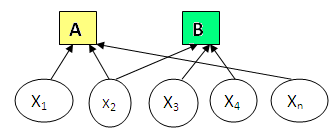
\includegraphics[scale=0.5]{bap.PNG}}
\caption{Bipartite Attribute Affiliation Graph}
\label{fig 1}
\end{figure}

A Bipartite Attribute Affiliation Graph is denoted as $B(X,C,M)$,
with $X$ as the nodes, $C$ as the attribute value and $M$ denotes
the directed edge from $X$ to $C$ if node $X$ has attribute
value $C$. The problem now is to create a set of communities
$S = S_1, S_2, ..., S_k$ given $B(X,C,M)$. A parameter $p_c$ is
assigned to an attribute value $c \in C$. This is for calculating
the probability that a node $x_i$ has the attribute value $c$. This
can also be called the probability that a node $x_i$ belongs to
the same community as another $x_j$ having the value of a
particular attribute as $c$. The $P_A(i, j)$ denotes that the nodes
$i, j$ belong to the same community $A$. This can be shown by
the below equation.

\begin{equation}
P_A(i,j) = 1 - \prod_{c \in M_i \cap M_j} (1 - p_c)
\end{equation} 

Where,

\begin{itemize}
\item $M_i$ = node $i$ has membership to attribute value $c$.
\item $M_j$ = node $j$ has membership to attribute value $c$.\\
\end{itemize}

In Eqn. 1, the value of $P_A(i, j)$ is set to $\varepsilon$, following
the BIGCLAM procedure the value of $\varepsilon$ can be set as
$2|E|/|V|(|V| - 1)$ [21].


\subsection{Calculate the latent weights of the attributes}

Every attribute has its own importance or strength in
determining the cluster to which the node should belong to,
this is denoted here formally as $F_{uC}$. This is the strength
that attribute $C$ has for node $u$ in determining its cluster.
Considering this membership strength the Eqn. 1 can be
modified as follows:

\begin{equation}
P_A(i,j) = 1 - exp(-F_{uC}.F_{vC}^T)
\end{equation}

$F_{uC}$ is the membership strength of a single attribute,
similarly it is assumed that every node $i$ has a attribute
membership vector $F_i$ which contains the membership
strengths to all attributes in the data. The modified probability
that nodes $i, j$ now share a cluster is Eqn 2.\\


The intuition behind the above formula is simple, Consider
a node having attribute values same as the attribute values
of another node, in such a case the likelihood of both
nodes belonging to a particular community increases. This
means that for each attribute a pair of nodes shares we
get an independent chance of grouping the nodes. Thus,
naturally, the more attributes a pair of nodes shares, the
higher the probability of sharing the same community and
being connected.\\


 
If $M_u \cap M_v = 0$ then $P(u,v) = \varepsilon$ this is done to consider
cases where nodes might not share attributes but still are
connected. $F_u$ is the vector that denotes the strengths of
association of a node $u$ with each attribute community in the network.
The task is to find the matrix of memberships $F$ that
maximizes the likelihood of generating the graph $G(V,E)$.
The log-likelihood of this is Eqn. 5. The Gradient update
algorithm is used to find the value of $F$ as shown in Eqn. 6 \\

\begin{equation}
l(F) = \sum_{u,v \in E} log(1 - \exp(-F_u.F_v^T)) - \sum_{u,v \notin E}(F_u.F_v^T)
\end{equation}
\begin{equation}
\bigtriangledown l(F_u) = \sum_{v \in N(u)} F_v \frac{\exp(-F_u.F_v^T)}{1 - \exp(-F_u.F_v^T)} - \sum_{v \notin N(u)} F_v
\end{equation}

\textbf{Decide Community Affiliation:} The membership strengths
matrix $F$ is computed from above and the next step is to
determine a suitable threshold above which it is possible to
determine whether the node $i$ belongs to a community. This
threshold is $\delta$ set at $\sqrt{−log(1 - \varepsilon)}$ [21]. The initialization
isn't done using locally minimal neighborhoods approach of
BIG-CLAM \cite{aps:53} as entity annotated attributes are used to get
initial values of the membership strengths $F_i$. The value of
$F_{i,k}$ is 0 if attribute $k$ is present and 0 if absent.\\

$\textbf{Choosing the number of communities:}$ This is done by
procedure specified in \cite{aps:53} where the model is trained using
an initial value of K. Then we detect K communities on the
80\% of node pairs and then evaluate the likelihood on the hold
out set. The K with the best hold out likelihood is used.\\

\section{Experiments}
In this section, evaluation of the performance of the variant of BIG-CLAM and other state-of-the-art community detection methods is done. The data-set used in this work consists of an artificially generated network with node attributes created using the tool described in the work of  Christine Largeron \textit{et. al.} \cite{aps:55}. Community detection methods such as Louvain and Fastgreedy technique were not applied as the graph was directed.

\subsection{Dataset and Evaluation Criteria}
The Artificially generated data-set is described below. The comparison metrics used are Variation of information (VI), Normalized mutual information, Split-join distance, Rand index (RI) and Adjusted Rand index (ARI). NMI, RI and ARI are in the range (0 - 1) with higher value indicating better clustering. The split-join distance between partitions A and B is the sum of the projection distance of A from B and the projection distance of B from A and should be low. VI should also ideally have a low value.

\begin{table}[H]
\renewcommand{\arraystretch}{1.3}
\caption{Description of the dataset}
\label{table}
\centering
\begin{tabular}{|c|c|c|}
  \hline
\multicolumn{1}{|c|}{\textbf{Sr. No}} & \multicolumn{1}{c|}{\textbf{Parameter}} & \multicolumn{1}{c|}{\textbf{Value}} \\
  \hline
  1 & Node Attributes &  3 \\
   \hline
  2 & Nodes &  200 \\
   \hline
  3 & Communities &  4 \\
   \hline
  4 & Observed homophily &  0.74 \\
   \hline
  5 & Modularity &  0.51 \\
   \hline
  6 & Avg. Clustering Coeff &  0.33 \\
   \hline
  7 & Avg. Degree &  5 \\
   \hline
  8 & Edges &  500 \\
   \hline
  9 & Network Type &  Directed-Unweighted \\
  \hline
\end{tabular}
\end{table}

\begin{figure}[H]
\centering
\fbox{\includegraphics[scale=0.5]{dataset.png}}
\caption{Artificially generated Network dataset}
\end{figure}

\subsection{Experimental Results}

\subsubsection{InfoMap}
"infomap.community" detected multiple communities in the network with few nodes leading to the conclusion that it split large clusters. The clustering is of poor quality as seen in Fig.\ref{InfoMap} as observed in the performance metrics.

\begin{table}[H]
\renewcommand{\arraystretch}{1.3}
\caption{Results}
\label{table}
\centering
\begin{tabular}{|c|c|c|}
  \hline
\multicolumn{1}{|c|}{\textbf{Sr. No}} & \multicolumn{1}{c|}{\textbf{Parameter}} & \multicolumn{1}{c|}{\textbf{Value}} \\
  \hline
  1 & Execution Time &  0.6 secs \\
   \hline
  2 & Modularity &  0.567 \\
   \hline
  3 & Variation of information &  1.72 \\
   \hline
  4 & Normalized mutual information &  0.565 \\
   \hline
  5 & Split-join distance &  115 \\
   \hline
  6 & Rand index &  0.717 \\
   \hline
  7 & Adjusted Rand index &  0.231 \\
  \hline
   8 & Detected Communities &  22 \\
  \hline
\end{tabular}
\end{table}

\subsubsection{Leading Eigenvector}
"leading.eigenvector.community" has uncovered a community structure with less communities as seen in Fig.\ref{leadg} and its performance is good on the metrics. 

\begin{table}[H]
\renewcommand{\arraystretch}{1.3}
\caption{Results}
\label{table}
\centering
\begin{tabular}{|c|c|c|}
  \hline
\multicolumn{1}{|c|}{\textbf{Sr. No}} & \multicolumn{1}{c|}{\textbf{Parameter}} & \multicolumn{1}{c|}{\textbf{Value}} \\
  \hline
  1 & Execution Time &  0.53 secs \\
   \hline
  2 & Modularity &  0.551 \\
   \hline
  3 & Variation of information &  0.88 \\
   \hline
  4 & Normalized mutual information &  0.67 \\
   \hline
  5 & Split-join distance &  74 \\
   \hline
  6 & Rand index &  0.795 \\
   \hline
  7 & Adjusted Rand index &  0.510 \\
  \hline
   8 & Detected Communities &  6 \\
  \hline
\end{tabular}
\end{table}

\subsubsection{Label Propagation}
"label.propagation.community" has detected low number of communities as seen in Fig.\ref{labelp}. Performance of this technique is better than other approaches. 

\begin{table}[H]
\renewcommand{\arraystretch}{1.3}
\caption{Results}
\label{table}
\centering
\begin{tabular}{|c|c|c|}
  \hline
\multicolumn{1}{|c|}{\textbf{Sr. No}} & \multicolumn{1}{c|}{\textbf{Parameter}} & \multicolumn{1}{c|}{\textbf{Value}} \\
  \hline
  1 & Execution Time &  0.06 secs \\
   \hline
  2 & Modularity &  0.545 \\
   \hline
  3 & Variation of information &  0.597 \\
   \hline
  4 & Normalized mutual information &  0.778 \\
   \hline
  5 & Split-join distance &  35 \\
   \hline
  6 & Rand index &  0.91 \\
   \hline
  7 & Adjusted Rand index &  0.81 \\
  \hline
   8 & Detected Communities &  8 \\
  \hline
\end{tabular}
\end{table}

\subsubsection{Walktrap}
"walktrap.community" uncovers a community structure with higher modularity as seen in Fig.\ref{walkt}. Large number of small communities have been created and so this technique has low values on the performance metrics. 

\begin{table}[H]
\renewcommand{\arraystretch}{1.3}
\caption{Results}
\label{table}
\centering
\begin{tabular}{|c|c|c|}
  \hline
\multicolumn{1}{|c|}{\textbf{Sr. No}} & \multicolumn{1}{c|}{\textbf{Parameter}} & \multicolumn{1}{c|}{\textbf{Value}} \\
  \hline
  1 & Execution Time &  0.11 secs \\
   \hline
  2 & Modularity &  0.579 \\
   \hline
  3 & Variation of information &  1.32 \\
   \hline
  4 & Normalized mutual information &  0.548 \\
   \hline
  5 & Split-join distance &  76 \\
   \hline
  6 & Rand index &  0.777 \\
   \hline
  7 & Adjusted Rand index &  0.446 \\
  \hline
   8 & Detected Communities &  15 \\
  \hline
\end{tabular}
\end{table}

\subsubsection{Spinglass and Clique Percolation}
"spinglass.community" detects high number of communities and has low values on VI, Split join and ARI metrics. Hence clustering quality is low as seen in Fig.\ref{sping}. Clique percolation with $k=3$ detected community structure given in as seen in Fig.\ref{cliquep} but 10\% of the nodes were unclassified.

\begin{table}[H]
\renewcommand{\arraystretch}{1.3}
\caption{Results}
\label{table}
\centering
\begin{tabular}{|c|c|c|}
  \hline
\multicolumn{1}{|c|}{\textbf{Sr. No}} & \multicolumn{1}{c|}{\textbf{Parameter}} & \multicolumn{1}{c|}{\textbf{Value}} \\
  \hline
  1 & Execution Time &  13.91 secs \\
   \hline
  2 & Modularity &  0.35 \\
   \hline
  3 & Variation of information &  1.12 \\
   \hline
  4 & Normalized mutual information &  0.638 \\
   \hline
  5 & Split-join distance &  94 \\
   \hline
  6 & Rand index &  0.772 \\
   \hline
  7 & Adjusted Rand index &  0.419 \\
  \hline
   8 & Detected Communities &  8 \\
  \hline
\end{tabular}
\end{table}

\subsection{Community Structures}
The figures below show the community structures uncovered by different approaches.

\begin{figure}[H]
  \begin{subfigure}[b]{0.3\linewidth}
    \includegraphics[width=\linewidth]{infomap.png}
    \caption{infomap}
    \label{InfoMap}
  \end{subfigure}
  \hfill %%
  \begin{subfigure}[b]{0.3\linewidth}
    \includegraphics[width=\linewidth]{leadg.png}
    \caption{Leading Eigenvector}
    \label{leadg}
  \end{subfigure}
\caption{Community structures in Network}
\end{figure}


\begin{figure}[H]
  \begin{subfigure}[b]{0.3\linewidth}
    \includegraphics[width=\linewidth]{labelp.png}
    \caption{Label propagation}
    \label{labelp}
  \end{subfigure}
  \hfill %%
  \begin{subfigure}[b]{0.3\linewidth}
    \includegraphics[width=\linewidth]{walkt.png}
    \caption{Walktrap}
    \label{walkt}
  \end{subfigure}
 \caption{Community structures in Network}
\end{figure}

\begin{figure}[H]
  \begin{subfigure}[b]{0.3\linewidth}
    \includegraphics[width=\linewidth]{sping.png}
    \caption{Spinglass}
    \label{sping}
  \end{subfigure}
  \hfill %%
  \begin{subfigure}[b]{0.3\linewidth}
    \includegraphics[width=\linewidth]{cliquep.png}
    \caption{Clique Percolation}
    \label{cliquep}
  \end{subfigure}
  \caption{Community structures in Network}
\end{figure}

\subsection{Variation of BIGCLAM}
With the above experimental results as baselines, the variation of BIGCLAM approach suggested in the paper was applied. The attributes were used to create a Bipartite graph as given by Jure Lescovec \textit{et. al} \cite{aps:53}, however the key difference was that the nodes were now having edges with the attributes. Network topology was thus ignored and BIGCLAM now used the Non negative matrix factorization to calculate the strength of memberships of the nodes to the attributes. These would be used to decide memberships of nodes to communities. As seen in Fig.\ref{bigc} the hold out set has highest likelihood at $k=6$. One advantage of this approach was large communities were formed and so it was inferred that splitting into smaller communities was avoided. As BIGCLAM is highly scalable, the network of $10^5$ nodes can be processed efficiently.

\begin{table}[H]
\renewcommand{\arraystretch}{1.3}
\caption{Results}
\label{table}
\centering
\begin{tabular}{|c|c|c|}
  \hline
\multicolumn{1}{|c|}{\textbf{Sr. No}} & \multicolumn{1}{c|}{\textbf{Parameter}} & \multicolumn{1}{c|}{\textbf{Value}} \\
  \hline
  1 & Execution Time &  8.51 secs \\
   \hline
  2 & Maximum likelihood Estimate &  -1070 \\
  \hline
   3 & Detected Communities &  6 \\
  \hline
\end{tabular}
\end{table}

\begin{figure}[H]
\centering
\fbox{\includegraphics[scale=0.3]{bigc.png}}
\caption{Clustering Structure using Variant of BIGCLAM}
\label{bigc}
\end{figure}



\section{Conclusion}
Community detection using a joint model of node attributes and network topology is a challenging task as additional information has to be factored while maintaining efficiency criteria. The model implemented in this paper uses Non negative matrix factorization on Bipartite Attribute Affiliation model for community detection. This approach allows for nodes to have high membership strengths simultaneously to various attribute communities. This allows for creating nested, overlapping and hierarchical communities in networks. The intuition behind this technique is that if the number of attributes shared by two nodes are high then the nodes have a higher probability of belonging to a single community. As this approach is relying on the optimization principle of BIGCLAM hence it is possible to state that this method can also be scaled to large networks efficiently.    


